% !TeX program = pdfLaTeX
\documentclass[12pt]{article}
\usepackage{amsmath}
\usepackage{graphicx,psfrag,epsf}
\usepackage{enumerate}
\usepackage{natbib}
\usepackage{textcomp}
\usepackage[hyphens]{url} % not crucial - just used below for the URL
\usepackage{hyperref}
\providecommand{\tightlist}{%
  \setlength{\itemsep}{0pt}\setlength{\parskip}{0pt}}

%\pdfminorversion=4
% NOTE: To produce blinded version, replace "0" with "1" below.
\newcommand{\blind}{0}

% DON'T change margins - should be 1 inch all around.
\addtolength{\oddsidemargin}{-.5in}%
\addtolength{\evensidemargin}{-.5in}%
\addtolength{\textwidth}{1in}%
\addtolength{\textheight}{1.3in}%
\addtolength{\topmargin}{-.8in}%

%% load any required packages here



\usepackage{booktabs}
\usepackage{longtable}
\usepackage{array}
\usepackage{multirow}
\usepackage{wrapfig}
\usepackage{float}
\usepackage{colortbl}
\usepackage{pdflscape}
\usepackage{tabu}
\usepackage{threeparttable}
\usepackage{threeparttablex}
\usepackage[normalem]{ulem}
\usepackage{makecell}
\usepackage{xcolor}

\usepackage{booktabs}
\usepackage{longtable}
\usepackage{array}
\usepackage{multirow}
\usepackage{wrapfig}
\usepackage{float}
\usepackage{colortbl}
\usepackage{pdflscape}
\usepackage{tabu}
\usepackage{threeparttable}
\usepackage{threeparttablex}
\usepackage[normalem]{ulem}
\usepackage{makecell}

\begin{document}


\def\spacingset#1{\renewcommand{\baselinestretch}%
{#1}\small\normalsize} \spacingset{1}


%%%%%%%%%%%%%%%%%%%%%%%%%%%%%%%%%%%%%%%%%%%%%%%%%%%%%%%%%%%%%%%%%%%%%%%%%%%%%%

\if0\blind
{
  \title{\bf Effects without a Cause: The Search for Demographic Anomalies}

  \author{
        Mathew E. Hauer \thanks{Thanks y'all!} \\
    Department of Sociology, Florida State University\\
     and \\     Stephanie A. Bohon \\
    Department of Sociology, University of Tennessee - Knoxville\\
      }
  \maketitle
} \fi

\if1\blind
{
  \bigskip
  \bigskip
  \bigskip
  \begin{center}
    {\LARGE\bf Effects without a Cause: The Search for Demographic Anomalies}
  \end{center}
  \medskip
} \fi

\bigskip
\begin{abstract}
The proliferation of data, modern computing advances, and powerful
statistical algorithms unlock the potential search for hidden,
previously un- or understudied demographic anomalies. Here, we
demonstrate how demographers can use causal inference techniques to
identify anamolies by investigating US state-level fertility and
mortality time series since 1999 to uncover the hidden baby booms/busts
and mortality plagues?/non-plauges?. We find 38 states exhibited at
least one mortality anomaly, totalling more than 318k anomalous deaths
and an additional 6 states exhibited at least one mortality non-plague?
totalling 164k protective deaths. 12 states exhibited baby busts,
totalling more than 240k missing births and an additional 11 states
exhibited baby booms totalling more than 134k additional births. These
results suggest the widespread detection of demographic anomalies. Our
analysis does not examine the \emph{causes} of these anomalies and our
results point to important further research on the causes of anomalous
demographic behavior.\\
\end{abstract}

\noindent%
{\it Keywords:} mortality, fertility, causal inference
\vfill

\newpage
\spacingset{1.45} % DON'T change the spacing!

\newpage

\hypertarget{introduction}{%
\section{Introduction}\label{introduction}}

The proliferation of data, advances in high performance (``super'')
computing, and the development of powerful statistical algorithms mark
the era of ``Big Data'' or data science
\citep{van2016data, zikopoulos2011}, with the potential for researchers
to find hidden or understudied social phenomena
\citep{bohon2018demography}. While the availability of Big Data and high
performance computing allows novel exploration of data through causal
inference
\citep{bohon2018demography, rcausalimpact, shiffrin2016drawing},
relatively few studies utilize causal inference techniques in the study
of demographic phenomena. However, understanding social phenomena using
these advances reveals important insights into society
\citep{angrist1989lifetime, mas2009peers} and allows us to better
monitor population trends \citep{nobles2019, torche2015hidden}.

Causal inference, in its most common usage, is an attempt to uncover the
underlying mechanism that results in changes in a phenomenon and have a
long history approaches in social sciences \citep{grimmer2015ppsp}.
Often, the identification of a casual mechanism requires either a
randomized control trial (RCT) or expert knowledge applied to a natural
experiment. For population-level analysis, expensive RCTs usually
preclude their widespread adoption \citep{west2008ajph}. Using natural
experiments provide less certainty about causation and fewer
opportunities to replicate work but they provide important and
widespread insights such as the determinants of migration, however,
provides important and more widespread insights on the determinants of
migration after Hurricane Katrina in 2006
\citep{fussellRecoveryMigrationCity2014, horiDisplacementDynamicsSouthern2009},
mini baby booms after electrical blackouts \citep{fetzer2018jpe}, and
the highly publicized estimates of excess mortality after Hurricane
Maria in Puerto Rico in 2016
\citep{kishore2018mortality, santos2018use}. Both RCTs and natural
experiments follow traditional, hypothesis testing, inductive scientific
paradigms where a question is first posed and scientists generate or
find data to answer the question. Such approaches, while extensively
utilized and time-tested, are likely to miss important phenomena that
might go unnoticed.

Both RCTs and natural experiments follow traditional hypothesis
testing--inductive scientific paradigms where a question is first posed
and scientists generate or find data to answer the question. Such
approaches, while extensively utilized and time-tested, are likely to
miss important phenomena that might go unnoticed. Data scientists are
rethinking these approaches and have re-envisioned causal inference as a
machine learning technique that allows big data researchers to move from
correlations that have been established with good accuracy to making
strong conclusions about the underlying mechanisms that produce these
correlations \citep{pearl2018book}.

Abductive modeling is the movement from the inductive to the deductive,
and sometimes back and forth, to reach conclusions
\citep{bryant2014realm} or ``inferring cause from effect''
\citep{Crowder2017}. In situations with large data sets, an abductive
approach is far superior to deductive hypothesis testing, as p-values
with an extremely large number of cases are far from revealing
\citep{head2015extent, nuzzo2014scientific} and we do not want to make
purely inductive inferences from data of questionable generalizability
\citep{ruggles2014big}. Owing to the long history of big data sets in
demographic research (one of the original ``big data'' resources
\citep{ruggles2014big}), the rich demographic data available in the
United States make the potential revelation of interesting and important
demographic phenomena not only possible, but extremely plausible -- even
if identification of the phenomena occurs without identifying the
underlying cause. In other sciences, the identification of effects
without causes has led to new theories of galactic migration of planets
and other breakthroughs \citep{gomes2005n}.

In this paper, we use modern statistical outlier detection algorithms
\citep{chen1993joint} on nearly twenty years of mortality and fertility
data at the US state-level to identify anomalous demographic behavior.
In essence, we identify \emph{effects without knowledge of the cause}.
We ask two questions regarding demographic anomalies: What are the
hidden baby booms/busts and mortality spikes/dips in the United States
over the last twenty years? We do not necessarily know the causes of
these anomalies but identifying them allows scientists with more
detailed knowledge of local population dynamics, state-level policy
making, or macro-economics to explain these phenomena post-hoc. From
explanations of phenomena that may have previously gone unnoticed,
demographers may be able to better forecast populations and provide
policy solutions for impending problems.

\hypertarget{materials-and-methods}{%
\section{Materials and Methods}\label{materials-and-methods}}

\hypertarget{method}{%
\subsection{Method}\label{method}}

We use a statistical time series outlier detection algorithm
\citep{chen1993joint}, implemented in the R programming language
\citep{rcore} via the tsoutliers package \citep{tsoutliers2019}. This
algorithm iteratively uses ARIMA models to 1) produce a counter-factual
time series to initially detect an outlier or anomaly, and 2) refit the
ARIMA with the outliers removed. Here we briefly summarize and describe
the method.

Often, the behavior of a time series can be described and summarized in
ARIMA models. If a series of values, \(y_t^*\), is subject to \(m\)
interventions or outliers at time points \(t_1,t_2,…,t_m\), then
\(y_t^*\) can be defined as

\[y_t^* = \sum_{j=1}^{m} \omega_jL_j(B)I_t(t_j) + \frac{\theta(B)}{\phi(B)\alpha(B)}\alpha_t\]

Where \(I_t(t_j)\) is an indicator variable with a value of 1 at
observation \(t_j\) and where the \(j\)th outlier arises, \(\phi(B)\) is
an autoregressive polynomial with all roots outside the unit circle,
\(\theta(B)\) is a moving average polynomial with all roots outside the
unit circle, and \(\alpha(B)\) is an autoregressive polynomial with all
roots on the unit circle.

We examine three types of outliers at time point \(t_m\): 1) additive
outliers (AO), defined as \(L_j(B)=1\); 2) level shift outliers (LS),
defined as \(L_j(B) = 1/(1-B)\); and 2) temporary change outliers (TC),
defined as \(L_j(B) = 1/(1-\delta B)\).

Colloquially, additive outliers arise when a single event causes the
time series to unexpectedly increase/decrease for a single time period;
level shift outliers arise when an event causes the time series to
unexpectedly increase/decrease for multiple time periods; and temporary
change outliers arise when an event causes the time series to
unexpectedly increase/decrease with lingering effects that decay over
multiple time periods.

An outlier is detected using a regression equation

\[ \pi(B)y_t^* \equiv \hat{e} = \sum_{j=1}^m \omega_j \pi(B)L_j(B)I_t(t_j) + \alpha_t \]

where \(\pi(B)=\sum_{i=o}^{inf} \pi_iB^i\). The identification of
outliers then involves a three step process to (1) identify all
potential outliers, \(t_j\) and \(L_j (B)\), (2) joint estimates of
model parameters and outlier effects are computed to identify
potentially spurious outliers, and (3) the outliers and effects are
re-estimated without spurious outliers. Of importance here is step 2,
which relies on some critical value above which an outlier at time point
m is considered spurious. Based on Chen and Liu's
\citeyearpar{chen1993joint} recommendation, we set a critical value of
3.5 which generally minimizes the possibility of Type I errors or false
positive outliers. Outliers are reported using a simple t-statistic.

\hypertarget{data}{%
\subsection{Data}\label{data}}

We search for demographic anomalies using the Center for Disease Control
and Prevention's online WONDER monthly fertility (2003-2017) and
mortality databases (1999-2016) for all fifty states and the District of
Columbia \citep{CDC_fert07, CDC_mort}. These data sets contain every
birth and death record in the United States over the time periods of
interest, representing the universe of both mortality and fertility data
in the US. These data are considered the ``gold standard'' of data
collections \citep{mahapatra2007civil} and have been considered
``complete'' since 1968 \citep{hetzel2016us}. We search over each state
equivalent's (n=51) mortality (n=228) and fertility (n=180) monthly time
series for a total of 20,808 state-months of data.

\hypertarget{results}{%
\section{Results}\label{results}}

We detect numerous anomalous mortality and fertility events at the US
state-level since 1999. A full listing of these anomalies can be found
in the \textbf{Supplementary Materials}. We begin with a summary of the
anomalies we detect and then we highlight highly significant mortality
and fertility anomalies across all three types of outliers (Additive
Outliers, Level Shift Outliers, and Temporary Change Outliers) with
plausible explanations. Finally, we highlight two strong anomalies that
bely explanation.

\hypertarget{overall-anomalies}{%
\subsection{Overall Anomalies}\label{overall-anomalies}}

\textbf{\autoref{sumtable}} reports the overall stuff.

\begin{table}

\caption{\label{tab:unnamed-chunk-1}\textbf{Summary by Anomaly Type and Demographic Component.} n refers to the number of anomolies for each type and demogrpahic component, States refers to the number of unique states exhibiting that specific Type-demogrpahic component. \label{sumtable}}
\centering
\begin{tabular}[t]{lrrrr}
\toprule
\multicolumn{1}{c}{ } & \multicolumn{2}{c}{Fertility} & \multicolumn{2}{c}{Mortality} \\
\cmidrule(l{3pt}r{3pt}){2-3} \cmidrule(l{3pt}r{3pt}){4-5}
Type & n & States & n & States\\
\midrule
AO & 9 & 9 & 85 & 38\\
LS & 6 & 4 & 22 & 17\\
TC & 7 & 6 & 49 & 28\\
\bottomrule
\end{tabular}
\end{table}

\hypertarget{mortality}{%
\subsection{Mortality}\label{mortality}}

We begin with mortality for New York State
(\textbf{\autoref{fig:mortnewhamp}a}). We identify seven anomalies in
the mortality time series for New York, all with t-statistics in excess
of 3.91, making these anomalies highly significant. The algorithm
correctly identifies September 2001 as an additive outlier (2001:09
t=6.40) where mortality in that month was 1,628 higher than anticipated.
This mortality event is likely caused by the September 11 tragedy and
the detection of this mortality event provides confidence in our
detection of other anomalies.

In \textbf{\autoref{fig:mortnewhamp}a}, notice the strong level shift
(LS) that occurs in February 2004 (2004:02 t=5.59) which prevented
almost 870 deaths per month. This shift totals more than 144,000 averted
deaths compared to the counter-factual time series and is the single
largest mortality protective anomaly among all states. This translates
to 4.5\% fewer deaths than expected over the time period. What is
driving this mortality protection? What policies did NY put into place
that might have contributed to this considerable mortality reduction?
What environmental conditions may have changed? These are the kinds of
questions that arise from our analyses.

Contrast the mortality protection in New York with the enhanced
mortality in New Hampshire (\textbf{\autoref{fig:mortnewhamp}b}). Here
we detect two highly significant level shifts (LS) in the monthly
mortality data, first in April 2010 and again in November 2014 (2010:04
t=3.51; 2014:11 t=6.68). These anomalies suggest New Hampshire
experienced 9,700 more deaths (+14\% more than expected) in a seven-year
period beginning in early 2010. This is the single largest percentage
mortality increase/decrease we detected among all states. Not
coincidentally, NH has the second highest opioid-related mortality in
the US \citep{beetham2019access} and it is reasonable that we detect
this epidemic in our results.

\begin{figure}
\centering
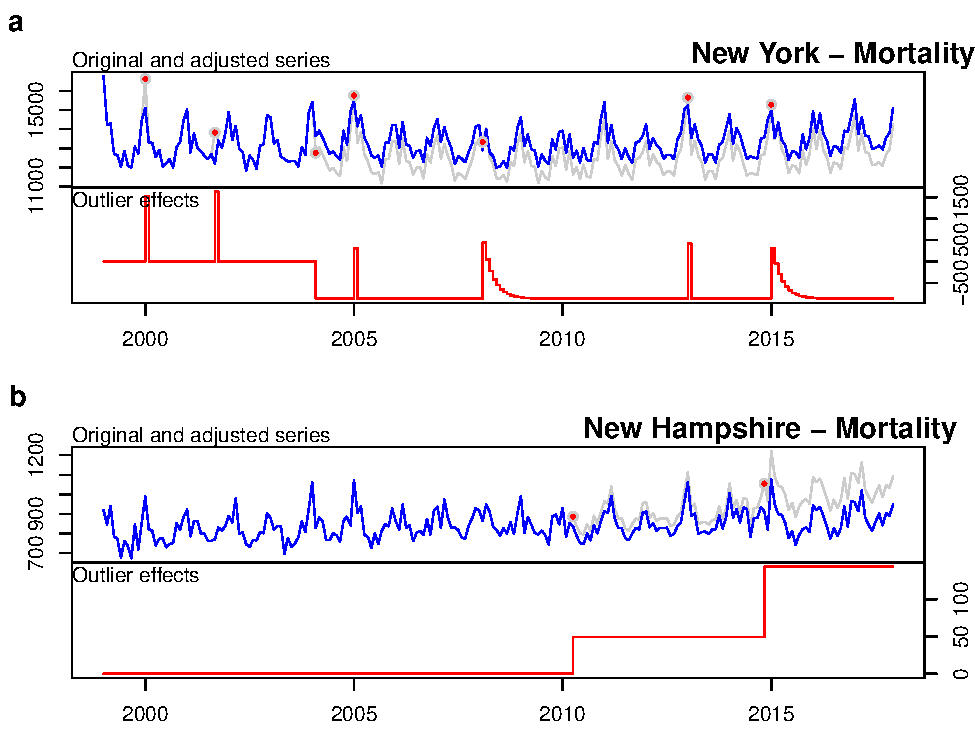
\includegraphics{manuscript_files/figure-latex/MortalityAnomalies-1.pdf}
\caption{\textbf{Anomaly Detection for New York (a) and New Hampshire (b) state mortality, 1999-2016.}
The top part of each panel contains the original time series (light
gray), the corrected, counter-factual time series in the absence of
anomalies (blue), and the red dots correspond to the onset of detected
anomalies. The bottom part of each panel contains the magnitude and type
of the outlier in red. In New York (a), we detect additive outliers (AO)
in January 2000, September 2001, January 2005, and January 2013;
temporary change (TC) outliers in February 2007 and January 2015; and a
level shift (LS) starting in February 2004. In New Hampshire (b), we
detect two outliers, both level shift outliers (LS) in April 2010 and
again in November 2014. These anomalies suggest New York experienced a
significant mortality event in September 2001 and New Hampshire
experienced approximately 9,700 more deaths than expected since 2010 or
14\% more deaths in the state over just seven years.
\label{fig:mortnewhamp}}
\end{figure}

\hypertarget{fertility}{%
\subsection{Fertility}\label{fertility}}

We begin with a clear temporary change (TC) outlier for fertility in
Louisiana (\textbf{\autoref{fig:fertla}a}). Here we detect two TC
outliers, nearly back-to-back in 2005 (2005:08 \emph{t} = -6; and
2005:10 \emph{t} = -5), coinciding with the destruction of Hurricane
Katrina from the same year. The migration associated with Hurricane
Katrina has garnered most of the attention of demographers
\citep{fussellRecoveryMigrationCity2014, horiDisplacementDynamicsSouthern2009},
but the hurricane had a very clear impact on fertility behaviors too,
creating a mini ``baby bust'' in Louisiana. We estimate 4,411 fewer
births in Louisiana compared to the counterfactual, likely attributable
to the Hurricane.

We also highlight a level shift (LS) outlier for fertility in
Connecticut. Here we detect a strong (\emph{t}= -3.71; -285
births/month) level shift toward lower fertility beginning in August
2009 (2009:08) that continues through the end of the period
(\textbf{\autoref{fig:fertla}b}). This LS toward lower fertility reduced
the \# of births by -28,752 or -8.57\% lower than the counterfactual
time series. The stock market crash of 2008, where the Dow Jones
Industrial Average had the largest single-day loss up to that point,
occured just 11 months before we detect a shift toward lower fertility.
We believe the trend toward lower fertility in August 2009 and the stock
market crash in September 2008 are linked.

\begin{figure}
\centering
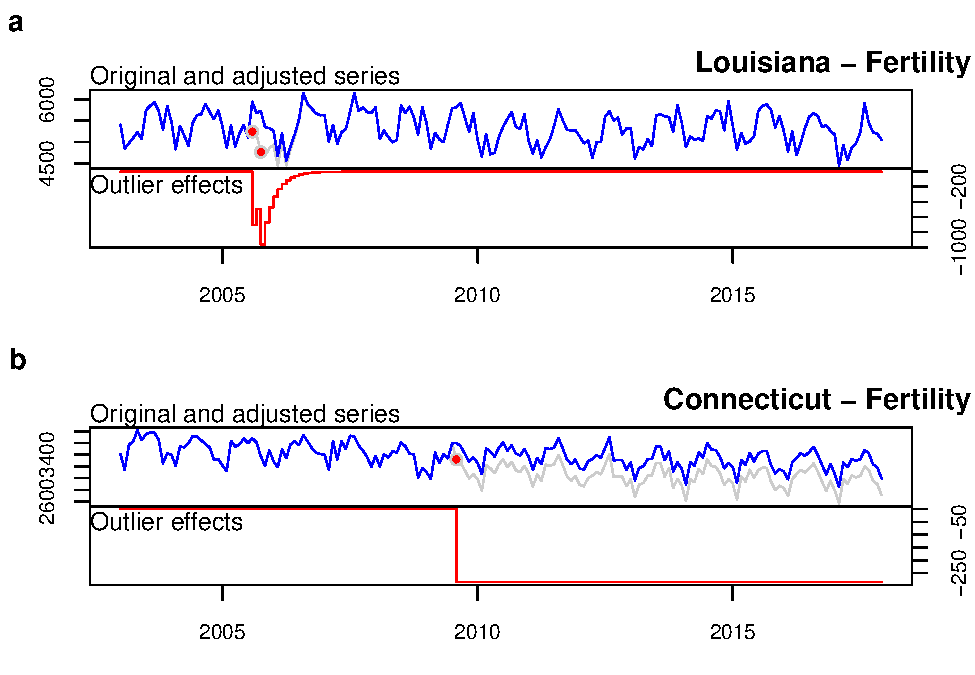
\includegraphics{manuscript_files/figure-latex/FertilityAnomalies-1.pdf}
\caption{\textbf{Anomaly detection in Louisiana (a) and Connecticut (b) state fertility, 2003-2018.}
In (a), we detect two outliers, back-to-back, likely resulting from
Hurricane Katrina in August and October 2005, representing a decrease of
more than 4,400 births due to the hurricane. In (b), we detect one
outlier, a level shift outlier (LS) in August 2009. We believe this
reduction is attributable to the stock market crash 11 months earlier.
\label{fig:fertla}}
\end{figure}

\hypertarget{interesting-anomalous-fertilitymortality-events}{%
\subsection{Interesting Anomalous Fertility/Mortality
events}\label{interesting-anomalous-fertilitymortality-events}}

In the examples above, we highlighted four fertility/mortality anomalies
with plausible explanations. In the case of New York and New Hampshire,
the mortality anomalies have plausible explanations. It seems likely
that New York's AO anomaly in September 2001 is caused by the 9/11
tragedy and the rise in New Hampshire's mortality starting in 2010 could
be linked to the opioid epidemic. Similarly, Louisiana's TC anomalies
seem linked to Hurricanes Katrina and Rita while the LS anomaly in
Connecticut's fertility appears linked to the Great Recession. However,
we detect numerous seemingly unexplainable demographic anomalies in
other states. \textbf{\autoref{fig:ferthawaii}} shows two such
unexplained anomalies.

In \textbf{\autoref{fig:ferthawaii}a} we identify a single additive
anomaly in Hawaiian fertility in May 2014. This is a strong anomaly with
a \emph{t}-statistic of 4.96, 14\% above the counter-factual time
series. This single, anomalous month is also the second highest monthly
births in the time series. We have no plausible explanation for this
anomaly. We do not believe this is simply a data error as the other
extreme values, September 2008 and February 2005 with the highest and
lowest recorded fertility respectively, were not identified as anomalous
events. Even if we were to assume this anomaly resulted from data entry
error, it remains an \emph{unaltered} data error in the Hawaiian monthly
fertility data.

This is contrast to \textbf{\autoref{fig:ferthawaii}b}, where we
identify a strange mortality reduction in Ohio (\emph{t}-stat: -4.27).
This LS is more than 1,100 deaths per month less than the counterfactual
time series, suggesting had nearly 40,000 fewer deaths since February
2015 than expected. This is the single-largest LS among all states. We
could not identify the potential policies Ohio might have put into place
to provide such a strong mortality protection.

\begin{figure}
\centering
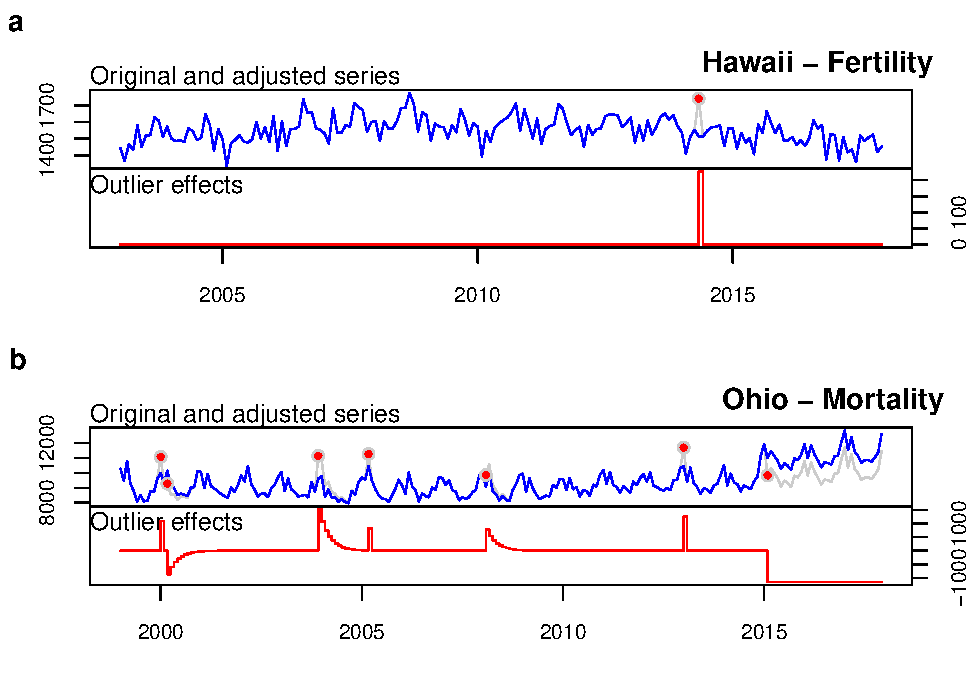
\includegraphics{manuscript_files/figure-latex/TrueAnomalies-1.pdf}
\caption{\textbf{Anomaly detection in Hawaii state fertility (a) and Ohio state mortality (b).}
Here we detect one outlier, an additive outlier (AO) in May 2014 in
Hawaii (a), representing a large, unexplainable 14\% increase in
expected births in that month. We also detect a strong level shift (LS)
reduction (b), representing a large, unexplainable reduction of nearly
40,000 deaths in Ohio. \label{fig:ferthawaii}}
\end{figure}

\newpage

\bibliographystyle{agsm}
\bibliography{mybibfile}

\end{document}
